\documentclass{beamer}
\usepackage[UKenglish]{babel}
\usepackage[UKenglish]{isodate}
\usepackage{graphicx}
\usepackage{subcaption}
\usepackage{tikz}
\usepackage{adjustbox}
\usepackage[backend=bibtex]{biblatex}
\usetikzlibrary{arrows}
\usetikzlibrary{positioning}

\author{Paulius Dilkas\\{\small Project Supervisor: Ciaran McCreesh}}
\title{Clique-Based Encodings for Graph Edit Distance}
\date{5th September 2017}
\institute{School of Computing Science}
\bibliography{../report.bib}

\begin{document}
\maketitle
\begin{frame}{The problem}
  \includegraphics[width=\textwidth]{ged.jpg} \\
  {\tiny\color{gray}Source: \cite{abu-aisheh_2016}}
  \pause
  \begin{figure}
    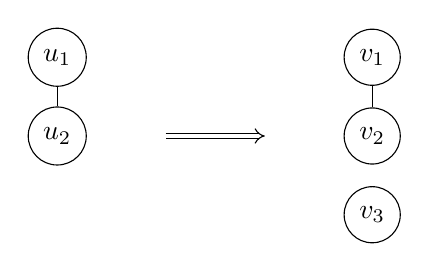
\begin{tikzpicture}
      \begin{scope}[every node/.style={circle,draw}]
        \node (a1) {$u_1$};
        \node (a2) [below of=a1] {$u_2$};
      \end{scope}
      \path (a1) edge node {} (a2);
      \begin{scope}[every node/.style={circle,draw},xshift=4 cm]
        \node (b1) {$v_1$};
        \node (b2) [below of=b1] {$v_2$};
        \node (b3) [below of=b2] {$v_3$};
      \end{scope}
      \path (b1) edge node {} (b2);
      \draw[-implies,double equal sign distance,shorten >=1cm,shorten <=1cm] (a2) -- (b2);
    \end{tikzpicture}
  \end{figure}
\end{frame}
\begin{frame}{Available operations}
  \begin{itemize}
  \item node insertion ($\epsilon \to v_i$),
  \item node deletion ($u_i \to \epsilon$),
  \item node substitution ($u_i \to v_j$),
  \item edge insertion ($\epsilon \to e_i$),
  \item edge deletion ($e_i \to \epsilon$),
  \item edge substitution ($e_i \to e_j$).
  \end{itemize}
\end{frame}
\begin{frame}{Use cases}
  \begin{columns}[t]
    \begin{column}{0.5\textwidth}
      \centering
      \includegraphics[width=\textwidth]{grec.jpg} \\
      {\tiny\color{gray}Source: International Symbol Recognition Contest\\[-7pt] GREC'2005} \\
      \vspace{1.15cm}
      \includegraphics[width=\textwidth]{muta.png} \\
      {\tiny\color{gray}Source: \cite{doi:10.1021/jm040835a}}
    \end{column}
    \begin{column}{0.5\textwidth}
      \centering
      \includegraphics[height=0.3\textheight]{protein.jpg} \\
      {\tiny\color{gray}Source: RCSB Protein Data Bank} \\
      \vspace{1cm}
      \includegraphics[height=0.3\textheight]{cmu.jpg} \\
      {\tiny\color{gray}Source: CMU/VASC Image Database}
    \end{column}
  \end{columns}
\end{frame}
\begin{frame}
  \begin{adjustbox}{max totalsize={0.9\textwidth}{0.9\textheight},center}
    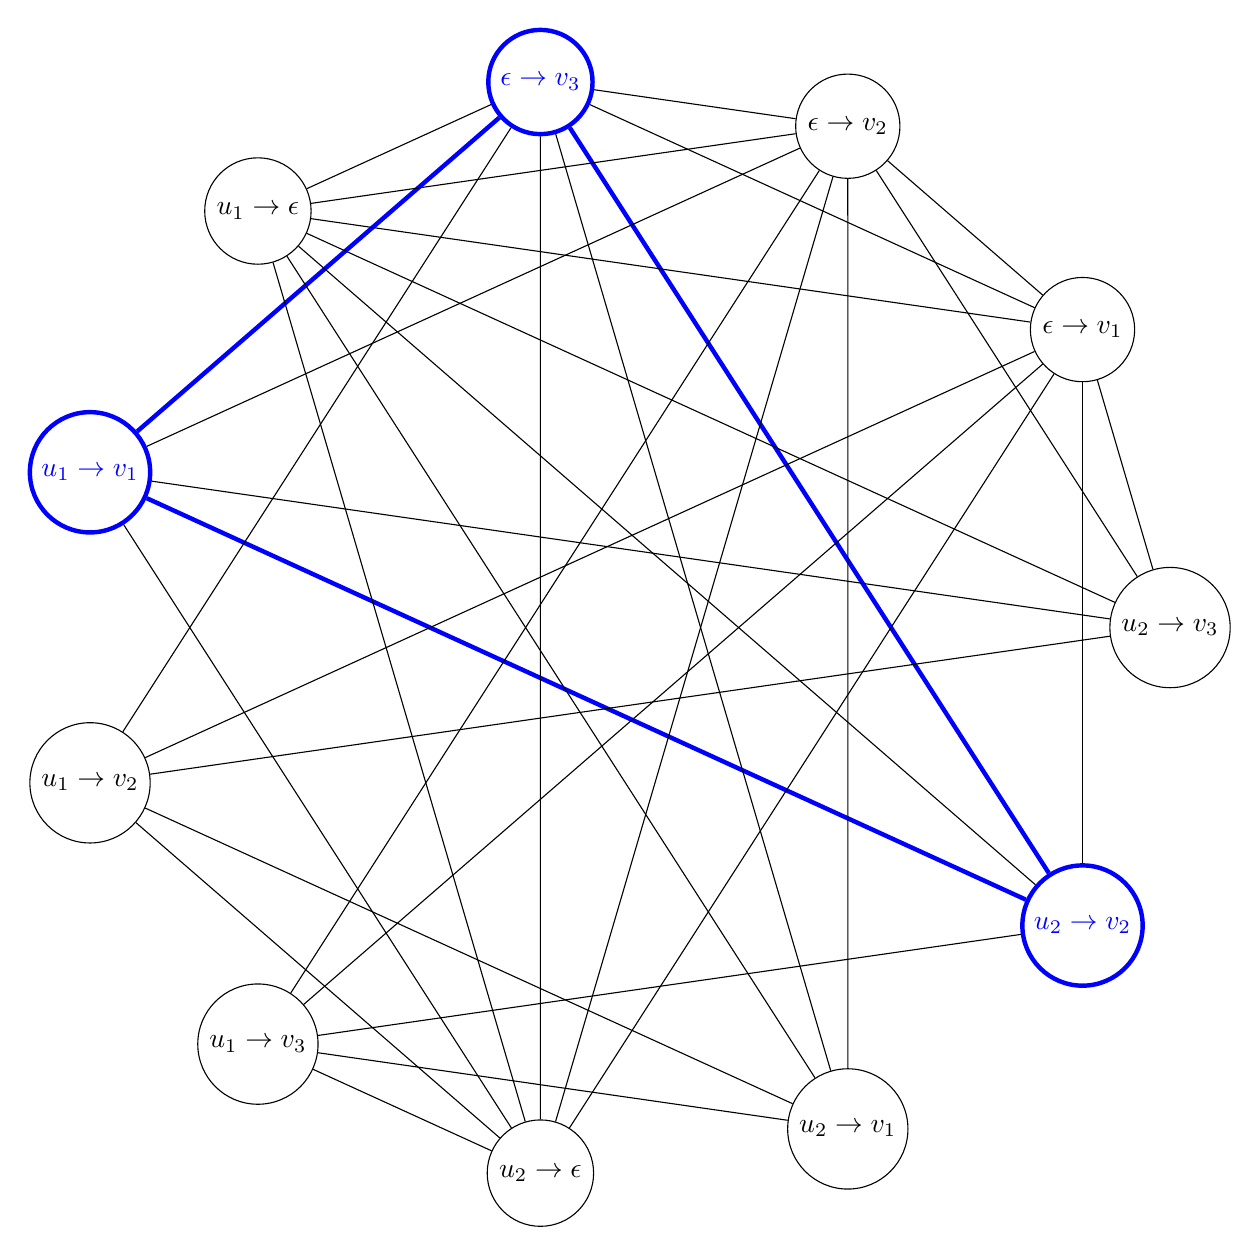
\begin{tikzpicture}
      \begin{scope}[every node/.style={circle,draw}]
        \node (i1) at (360/11 * 1:7cm) {$\epsilon \to v_1$};
        \node (i2) at (360/11 * 2:7cm) {$\epsilon \to v_2$};
        \node (i3) [color=blue,ultra thick] at (360/11 * 3:7cm) {$\epsilon \to v_3$};

        \node (d1) at (360/11 * 4:7cm) {$u_1 \to \epsilon$};
        \node (s11) [color=blue,ultra thick] at (360/11 * 5:7cm) {$u_1 \to v_1$};
        \node (s12) at (360/11 * 6:7cm) {$u_1 \to v_2$};
        \node (s13) at (360/11 * 7:7cm) {$u_1 \to v_3$};

        \node (d2) at (360/11 * 8:7cm) {$u_2 \to \epsilon$};
        \node (s21) at (360/11 * 9:7cm) {$u_2 \to v_1$};
        \node (s22) [color=blue,ultra thick] at (360/11 * 10:7cm) {$u_2 \to v_2$};
        \node (s23) at (360:7cm) {$u_2 \to v_3$};
      \end{scope}

      \begin{scope}[color=blue]
        \path (s11) [ultra thick] edge node {} (s22) edge node {} (i3);
        \path (s22) [ultra thick] edge node {} (i3);
      \end{scope}

      \path (i1) edge node {} (i2) edge node {} (i3) edge node {} (d1) edge node {} (s12) edge node {} (s13) edge node {} (d2) edge node {} (s22) edge node {} (s23);
      \path (i2) edge node {} (i3) edge node {} (d1) edge node {} (s11) edge node {} (s13) edge node {} (d2) edge node {} (s21) edge node {} (s23);
      \path (i3) edge node {} (d1) edge node {} (s12) edge node {} (d2) edge node {} (s21);
      \path (d1) edge node {} (d2) edge node {} (s21) edge node {} (s22) edge node {} (s23);
      \path (s11) edge node {} (d2) edge node {} (s23);
      \path (s12) edge node {} (d2) edge node {} (s21) edge node {} (s23);
      \path (s13) edge node {} (d2) edge node {} (s21) edge node {} (s22);
    \end{tikzpicture}
  \end{adjustbox}
\end{frame}
\begin{frame}{First encoding: weighted vertices \& edges}
  \begin{itemize}
  \item Each vertex represents an operation on nodes
  \item Weights of a vertex is equal to cost of operation
  \item Additional constraint: every node must be involved in some operation
  \end{itemize}
\end{frame}
%\begin{frame}
%  \begin{columns}
%    \begin{column}{0.3\textwidth}
%      \begin{figure}
%        \begin{tikzpicture}
%          \begin{scope}[every node/.style={circle,draw}]
%            \node (1) {$u_i \to v_i$};
%            \node (2) [below=1cm of 1] {$u_j \to v_j$};
%          \end{scope}
%          \path[color=red,ultra thick] (1) edge node {} (2);
%        \end{tikzpicture}
%      \end{figure}
%    \end{column}
%    \begin{column}{0.7\textwidth}
%      \begin{itemize}
%      \item Draw the edge if $u_i \ne u_j$, $v_i \ne v_j$
%      \item Weight of each edge is
%        \begin{itemize}
%        \item $\min(\text{substitution}, \text{deletion}+\text{insertion})$ if both edges exist,
%        \item otherwise cost of insertion/deletion or no cost as appropriate
%        \end{itemize}
%      \end{itemize}
%    \end{column}
%  \end{columns}
%\end{frame}
\begin{frame}{Second encoding: weighted vertices}
\begin{itemize}
\item Vertices represent ALL possible operations
\item Weights correspond to costs of operations
%\item Rules for when to draw an edge get more complicated...
\item Additional constraint: every node and edge must be involved in some operation
\item The graph is quadratically bigger than the first encoding
\end{itemize}
\end{frame}
\begin{frame}
  \begin{adjustbox}{max totalsize={0.9\textwidth}{0.9\textheight},center}
    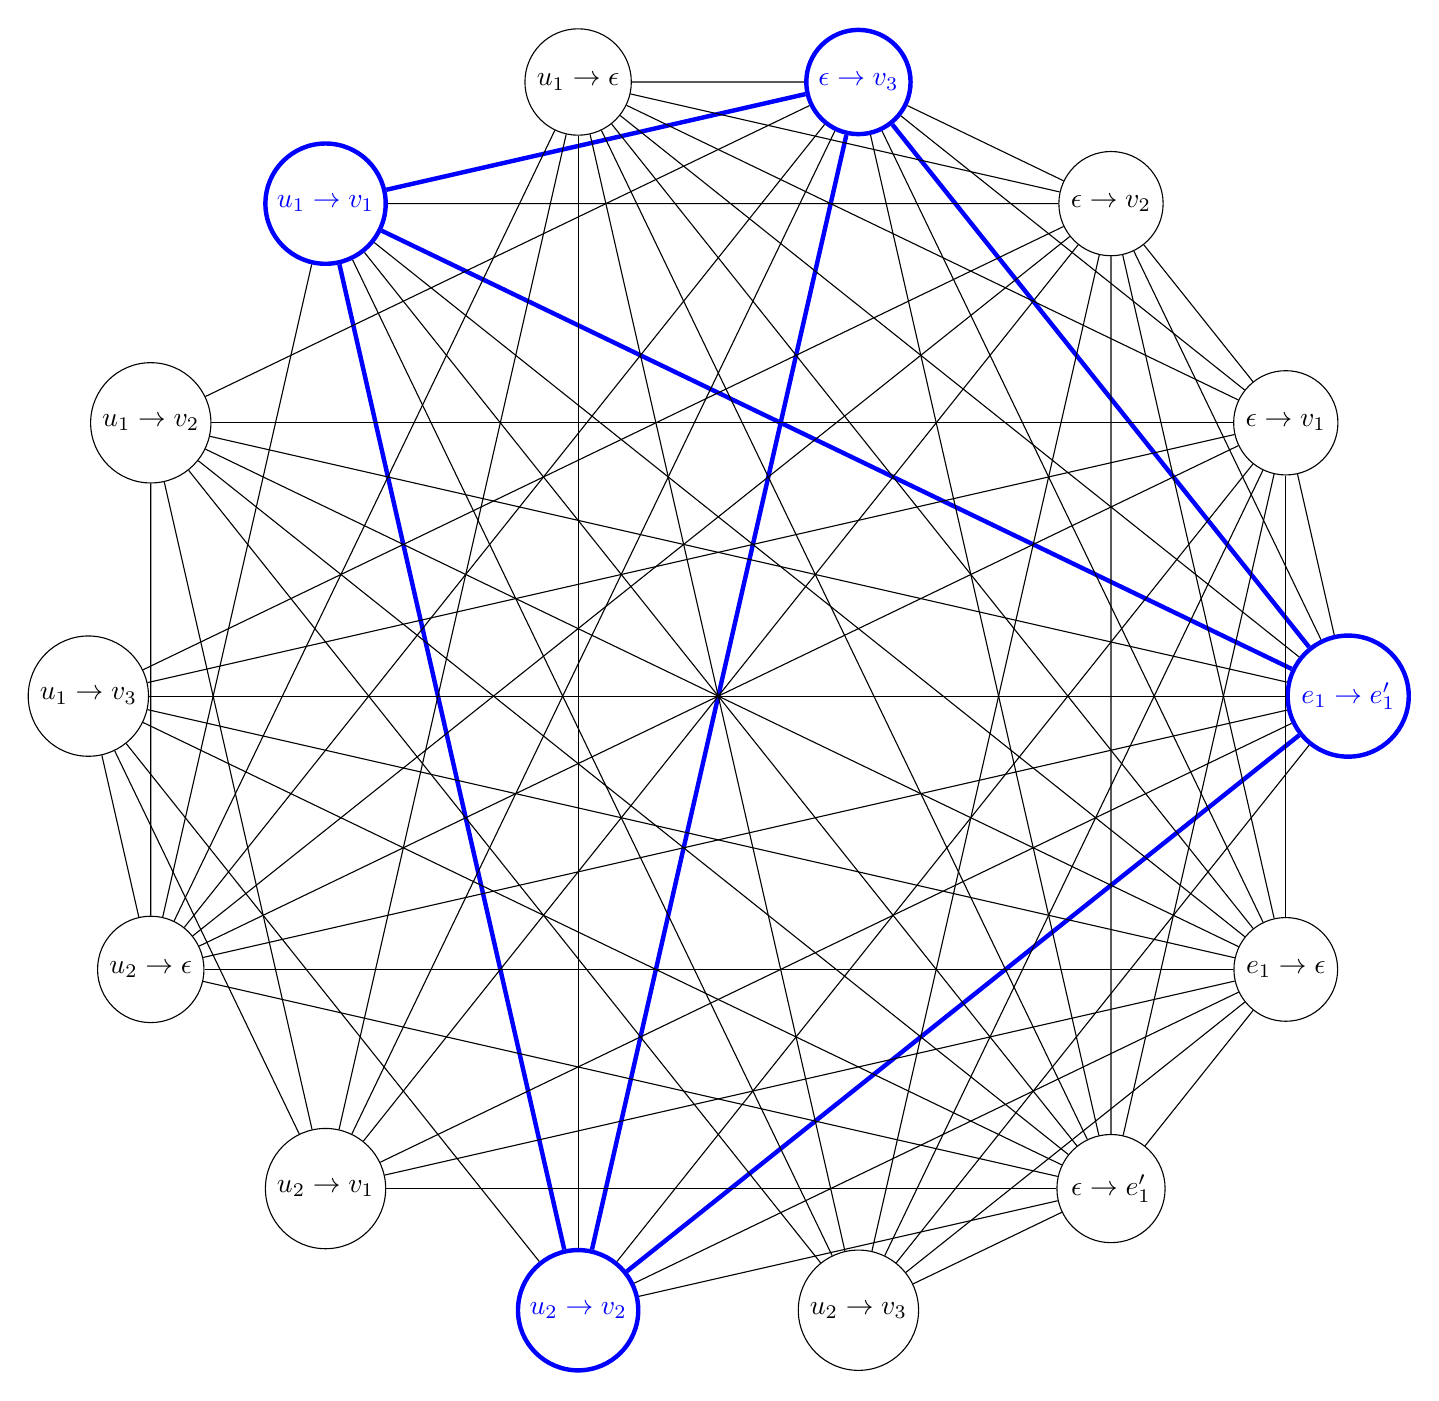
\begin{tikzpicture}
      \begin{scope}[every node/.style={circle,draw}]
        \node (vi1) at (360/14 * 1:8cm) {$\epsilon \to v_1$};
        \node (vi2) at (360/14 * 2:8cm) {$\epsilon \to v_2$};
        \node (vi3) [color=blue,ultra thick] at (360/14 * 3:8cm) {$\epsilon \to v_3$};

        \node (vd1) at (720/7:8cm) {$u_1 \to \epsilon$};
        \node (vs11) [color=blue,ultra thick] at ({720/7 + 360/14 * 1}:8cm) {$u_1 \to v_1$};
        \node (vs12) at ({720/7 + 360/14 * 2}:8cm) {$u_1 \to v_2$};
        \node (vs13) at ({720/7 + 360/14 * 3}:8cm) {$u_1 \to v_3$};

        \node (vd2) at (720/7 + 360/14 * 4:8cm) {$u_2 \to \epsilon$};
        \node (vs21) at ({720/7 + 360/14 * 4 + 360/14 * 1}:8cm) {$u_2 \to v_1$};
        \node (vs22) [color=blue,ultra thick] at ({720/7 + 360/14 * 4 + 360/14 * 2}:8cm) {$u_2 \to v_2$};
        \node (vs23) at ({720/7 + 360/14 * 4 + 360/14 * 3}:8cm) {$u_2 \to v_3$};

        \node (ei) at (2160/7:8cm) {$\epsilon \to e_1'$};
        \node (ed) at (2340/7:8cm) {$e_1 \to \epsilon$};
        \node (es) [color=blue,ultra thick] at (360:8cm) {$e_1 \to e_1'$};
      \end{scope}

      \begin{scope}[draw=blue]
        \path (vi3) [ultra thick] edge node {} (vs11) edge node {} (vs22) edge node {} (es);
        \path (vs11) [ultra thick] edge node {} (vs22) edge node {} (es);
        \path (vs22) [ultra thick] edge node {} (es);
      \end{scope}

      \path (vi1) edge node {} (vi2) edge node {} (vi3) edge node {} (vd1) edge node {} (vs12) edge node {} (vs13) edge node {} (vd2) edge node {} (vs22) edge node {} (vs23) edge node {} (ei) edge node {} (ed) edge node {} (es);
      \path (vi2) edge node {} (vi3) edge node {} (vd1) edge node {} (vs11) edge node {} (vs13) edge node {} (vd2) edge node {} (vs21) edge node {} (vs23) edge node {} (ei) edge node {} (ed) edge node {} (es);
      \path (vi3) edge node {} (vd1) edge node {} (vs12) edge node {} (vd2) edge node {} (vs21) edge node {} (ei) edge node {} (ed);
      \path (vd1) edge node {} (vd2) edge node {} (vs21) edge node {} (vs22) edge node {} (vs23) edge node {} (ei) edge node {} (ed) edge node {} (es);
      \path (vs11) edge node {} (vd2) edge node {} (vs23) edge node {} (ei) edge node {} (ed);
      \path (vs12) edge node {} (vd2) edge node {} (vs21) edge node {} (vs23) edge node {} (ei) edge node {} (ed) edge node {} (es);
      \path (vs13) edge node {} (vd2) edge node {} (vs21) edge node {} (vs22) edge node {} (ei) edge node {} (ed) edge node {} (es);
      \path (vd2) edge node {} (ei) edge node {} (ed) edge node {} (es);
      \path (vs21) edge node {} (ei) edge node {} (ed) edge node {} (es);
      \path (vs22) edge node {} (ei) edge node {} (ed);
      \path (vs23) edge node {} (ei) edge node {} (ed) edge node {} (es);
      \path (ei) edge node {} (ed);
    \end{tikzpicture}
  \end{adjustbox}
\end{frame}
\begin{frame}{Performance of the CP models}
  \includegraphics[scale=0.6]{../comparison.png}
\end{frame}
\begin{frame}{The algorithm}
  \begin{itemize}
  \item Branch and bound
  \item Lower bound function based on W. A. Tavares' colouring \cite{DBLP:phd/hal/tavares16}
  \item Bitsets for keeping track of vertices that can still be part of the clique
  \end{itemize}
\end{frame}
\begin{frame}{Performance on different datasets}
  \includegraphics[scale=0.6]{../ecdfs.png}
\end{frame}
\begin{frame}{Compared to other algorithms \cite{DBLP:conf/icpram/Abu-AishehRRM15}}
  \begin{itemize}
  \item DF-GED: optimal answers in 350 ms with 20-vertex graphs
  \item My algorithm: answers after 15 s up to 5\% higher than optimal for 15-vertex graphs
  \end{itemize}
  \begin{itemize}
  \item A*GED: fails to finish in 350 ms with most of 10-vertex graphs
  \item My algorithm: maximum running time is 195 ms, mean running time is 34.73 ms
  \end{itemize}
\end{frame}
\begin{frame}[allowframebreaks]{References}
  \printbibliography
\end{frame}
\begin{frame}
  \begin{block}{Contact details}
    Paulius Dilkas \\
    \url{2146879d@student.gla.ac.uk} \\
    or \url{paulius.dilkas@gmail.com}
  \end{block}
  \bigskip
  \begin{block}{Code and paper avalable at}
    \url{https://github.com/dilkas/graph-edit-distance}
  \end{block}
\end{frame}
\end{document}
